\documentclass[a4paper, 11pt, oneside]{report} 
\usepackage[utf8]{inputenc}
\usepackage[dutch]{babel}
\usepackage{amsmath}
\usepackage{amsfonts}
\usepackage{amssymb}
\usepackage{graphicx}
\usepackage{caption}
\usepackage[table,xcdraw]{xcolor}
\usepackage[toc,page]{appendix}
\usepackage{hyperref}
\usepackage{titlesec}
\usepackage{listings}
\usepackage{float}
\usepackage{tikz}
\usetikzlibrary{trees}
\usepackage{tikz-qtree}
\usepackage{graphicx}
\usepackage{fancyref}
\usepackage{wrapfig}
\usepackage{url}
\usepackage{pdflscape}
\usepackage{fancyvrb}
\usepackage{fancyhdr}
\graphicspath{ {Afbeeldingen/} }
\usepackage{subfig}
\usepackage{tabularx}
\usepackage{apacite}
\usepackage{longtable}
\usepackage{titlecaps}
%\usepackage[T1]{fontenc}
\usepackage{titlesec, blindtext, color}
\definecolor{gray75}{gray}{0.75}
\newcommand{\hsp}{\hspace{20pt}}
\usepackage{pdfpages}
\usepackage{afterpage}


\newcolumntype{L}[1]{>{\raggedright\arraybackslash}p{#1}}

\titleformat{\chapter}[hang]{\huge\bfseries}{\thechapter\hsp\textcolor{gray75}{|}\hsp}{0pt}{\Large\bfseries}

\def\figureautorefname{Figuur}
\def\sectionautorefname{Paragraaf}
\def\chapterautorefname{Hoofdstuk}
\def\tableautorefname{Tabel}
\DeclareRobustCommand{\VAN}[3]{#2} % set up for citation

%% Sets page size and margins 
\usepackage[a4paper,top=3cm,bottom=3cm,left=3cm,right=3cm,marginparwidth=1.75cm]{geometry}

\author{M.W.J. Berentsen}
\font\myfont=cmr12 at 40pt
\title{\myfont Drone meshnetwerk simulatie}
\usepackage{titling}

\newcommand{\subtitle}[8]{%
	\posttitle{%
		\par\end{center}
	\begin{center}\large#1\end{center}
	\vskip0.5em
	\begin{center}\large#2\end{center}
	\begin{center}\large#3\end{center}
	\begin{center}\large#4\end{center}
	\begin{center}\large#5\end{center}
	\begin{center}\large#6\end{center}
	\begin{center}\large#7\end{center}
	\begin{center}\large#8\end{center}
	\vskip0.5em}%
}

\subtitle{Software Design Document}{HAN Arnhem}{561399}{MWJ.Berentsen@student.han.nl}{Versie 1}{Alten Nederland B.V.}{Docent: J. Visch, MSc}{Assessor: ir. C.G.R. van Uffelen}

\setlength{\parindent}{0pt}
\setlength{\parskip}{5pt plus 2pt minus 1pt}



\hypersetup{colorlinks=true, urlcolor=red,citecolor=black,linkcolor=blue}  % Colours hyperlinks in blue, but this can be distracting if there are many links.
\setcounter{tocdepth}{2}



\begin{document}
\begin{figure}
	\begin{center}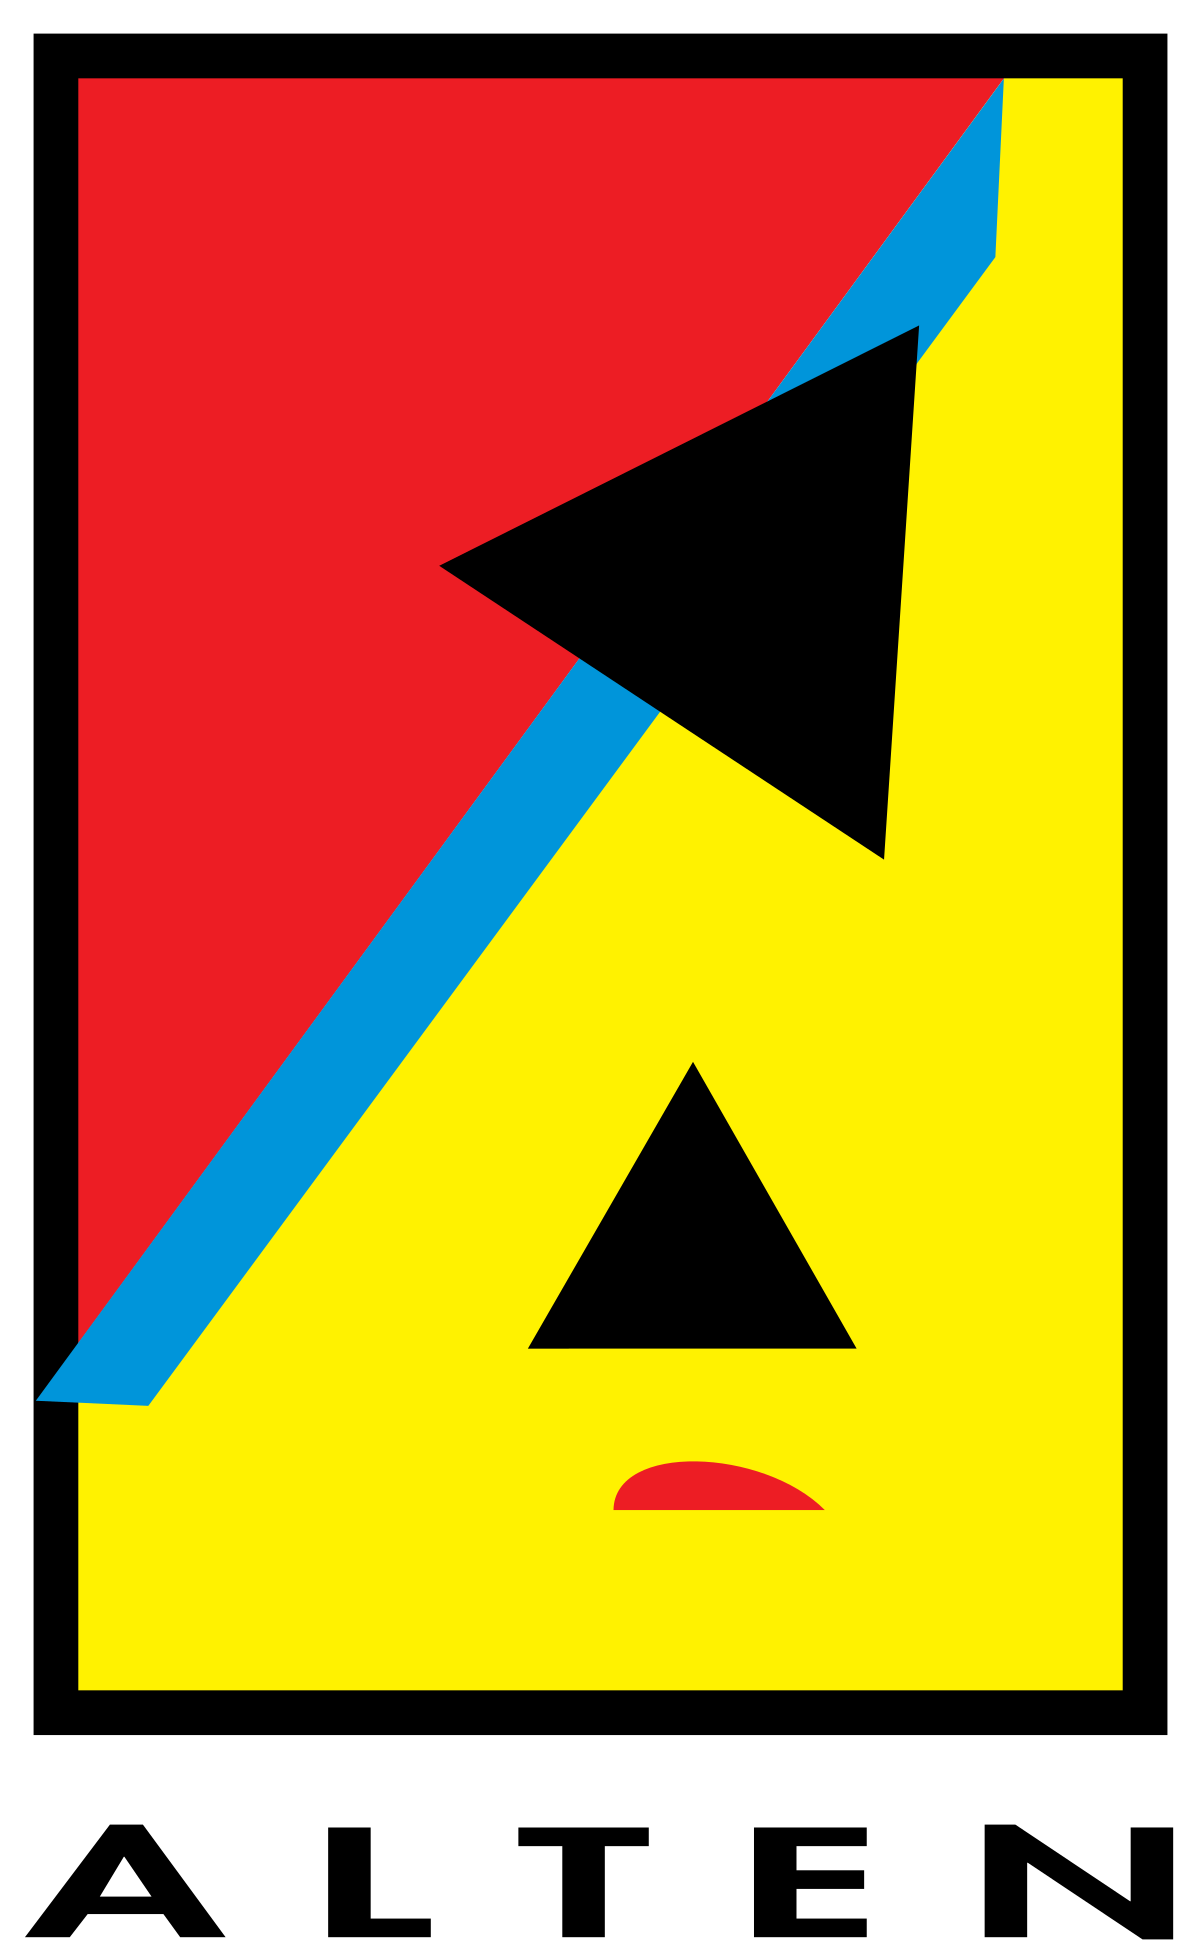
\includegraphics[scale=0.1]{alten}\end{center}
\end{figure}
\maketitle

%\section*{Voorwoord}
%\addcontentsline{toc}{section}{\protect\numberline{}Voorwoord}
%\pagebreak

%Geschikt voor minimaal 50 nodes; Kan slecht of geen signaal nabootsen

\tableofcontents
\clearpage


%\clearpage

%\section*{Samenvatting}
%\addcontentsline{toc}{section}{\protect\numberline{}Samenvatting}
%\pagebreak


\chapter{Inleiding}
\label{inleiding}
Het volgende verslag betreft de Software Requirements Specification voor de afstudeerstage van Maurice Berentsen (hierna: student).
Dit document volgt het document: \textit{"Software Design Description Template"} \cite{template:sdd}

Het beschrijft de hoe de uiteindelijke applicatie eruit zal zien en wat de functionaliteit hiervan zal zijn. Op de manier is het voor de student maar ook betrokken partijen duidelijk wat er gerealiseerd zal worden. Het verduidelijk de werking van de sub-componenten en de onderlinge relaties. 

\subsection{leeswijzer}
\label{inleiding:beschrijving:leeswijzer}
Eerst zal een korte beschrijving gegeven worden van het doel van dit document.Daarna wordt er door middel van een tabel een begrippenlijst toegelicht. In het tweede hoofdstuk is als eerste een component diagram te vinden waarin de functionaliteit van de verschillende componenten te vinden is en de manier waarop deze componenten met elkaar communiceren. Vervolgens is de algemene flow van het programma te zien, hierin wordt duidelijk welke stappen er onder water worden genomen als er een bepaalde actie wordt uitgevoerd. In hoofdstuk drie worden alle subsystemen duidelijk uitgewerkt en worden de ontwerpen van deze systemen uitgewerkt. 
\section{Begrippenlijst}
\label{inleiding:begrippenlijst}

% Please add the following required packages to your document preamble:
% \usepackage[table,xcdraw]{xcolor}
% If you use beamer only pass "xcolor=table" option, i.e. \documentclass[xcolor=table]{beamer}
\begin{table}[H]
\centering

\label{begrippen}
\begin{tabular}{|l|l|}
\hline
\rowcolor[HTML]{C0C0C0}
Term        & Omschrijving                                                         \\ \hline
term        & Omschrijving                                                      	\\ \hline

\end{tabular}
\caption{Begrippenlijst}
\end{table}

\chapter{Architectural Overview}
\label{architectural}
In het component diagram \autoref{fig:packagediagram} op de volgende pagina is te zien dat bepaalde componenten voorzien zijn van een andere kleur. 
De groene kleur betekend dat het component voorzien is door gazebo.
De rode en blauw kleur zijn gegeneerd door ROS waarbij de rode een rosservice zijn en de blauwe een rostopic.
Op het hoogste niveau is het diagram te verdelen in vier groepen.

\textbf{Communication} is het component die de beslissingen neemt voor de communicatie.
Het heeft de intelligentie om het netwerk in kaart te brengen en te routeren.
Daarnaast is het in staat om een beslissing te nemen om een verzoek te sturen om de drone te verplaatsen.
Tenslotte bevat het meerdere berichten die gebruikt om het netwerk te kunnen onderhouden en op te bouwen.    

\textbf{Drone} is op dit moment een leeg component waar alleen een high level interface aanwezig is die de mogelijkheid biedt om de huidige locatie van een drone terug te geven of een nieuwe locatie als doel te geven aan de drone. 

\textbf{Gazebo} is de plek waar de virtualisatie van de drone plaats vindt.
Er kunnen virtuele router of gateway drones gemaakt worden die voorzien zijn van een virtuele arduino ingeladen met de juiste software en een virtuele drone motor.
Deze worden als model plug-in gekoppeld aan de drone in een gesimuleerde wereld waar Gazebo vervolgens physics op de drones kan uitvoeren. 

\textbf{ROS} is het component waar de simulatie van de communicatie plaats vindt.
Er is een virtuele NRF24 om te communiceren met andere nodes in het netwerk.
De aanwezige WirelessSignalSimulator zorgt dat dit realistisch gebeurd door alleen communicatie uit te voeren als dit volgens de voorwaarden mag.
Dit bepaald de simulator op basis van informatie die het krijgt van Gazebo en de NRF.
Tenslotte is er een DroneManager aanwezig die een interface aanbiedt via ros voor de ontwikkelaar om verbinding te maken met de gateways uit het netwerk.

\textbf{Arduino} is het component die zich onderscheid in twee rollen, een Arduino kan de rol van gateway hebben of de rol van router in de het meshnetwerk.

\textbf{NRF24} is het gebruikte component om draadloze communicatie mogelijk te maken. Het is voorzien van een driver in de vorm van een low level interface en bied zich aan via een high level interface voor communicatie.

Na het component diagram zal elke subcomponent kort toegelicht worden


\begin{landscape}
	\begin{figure}[p]%
		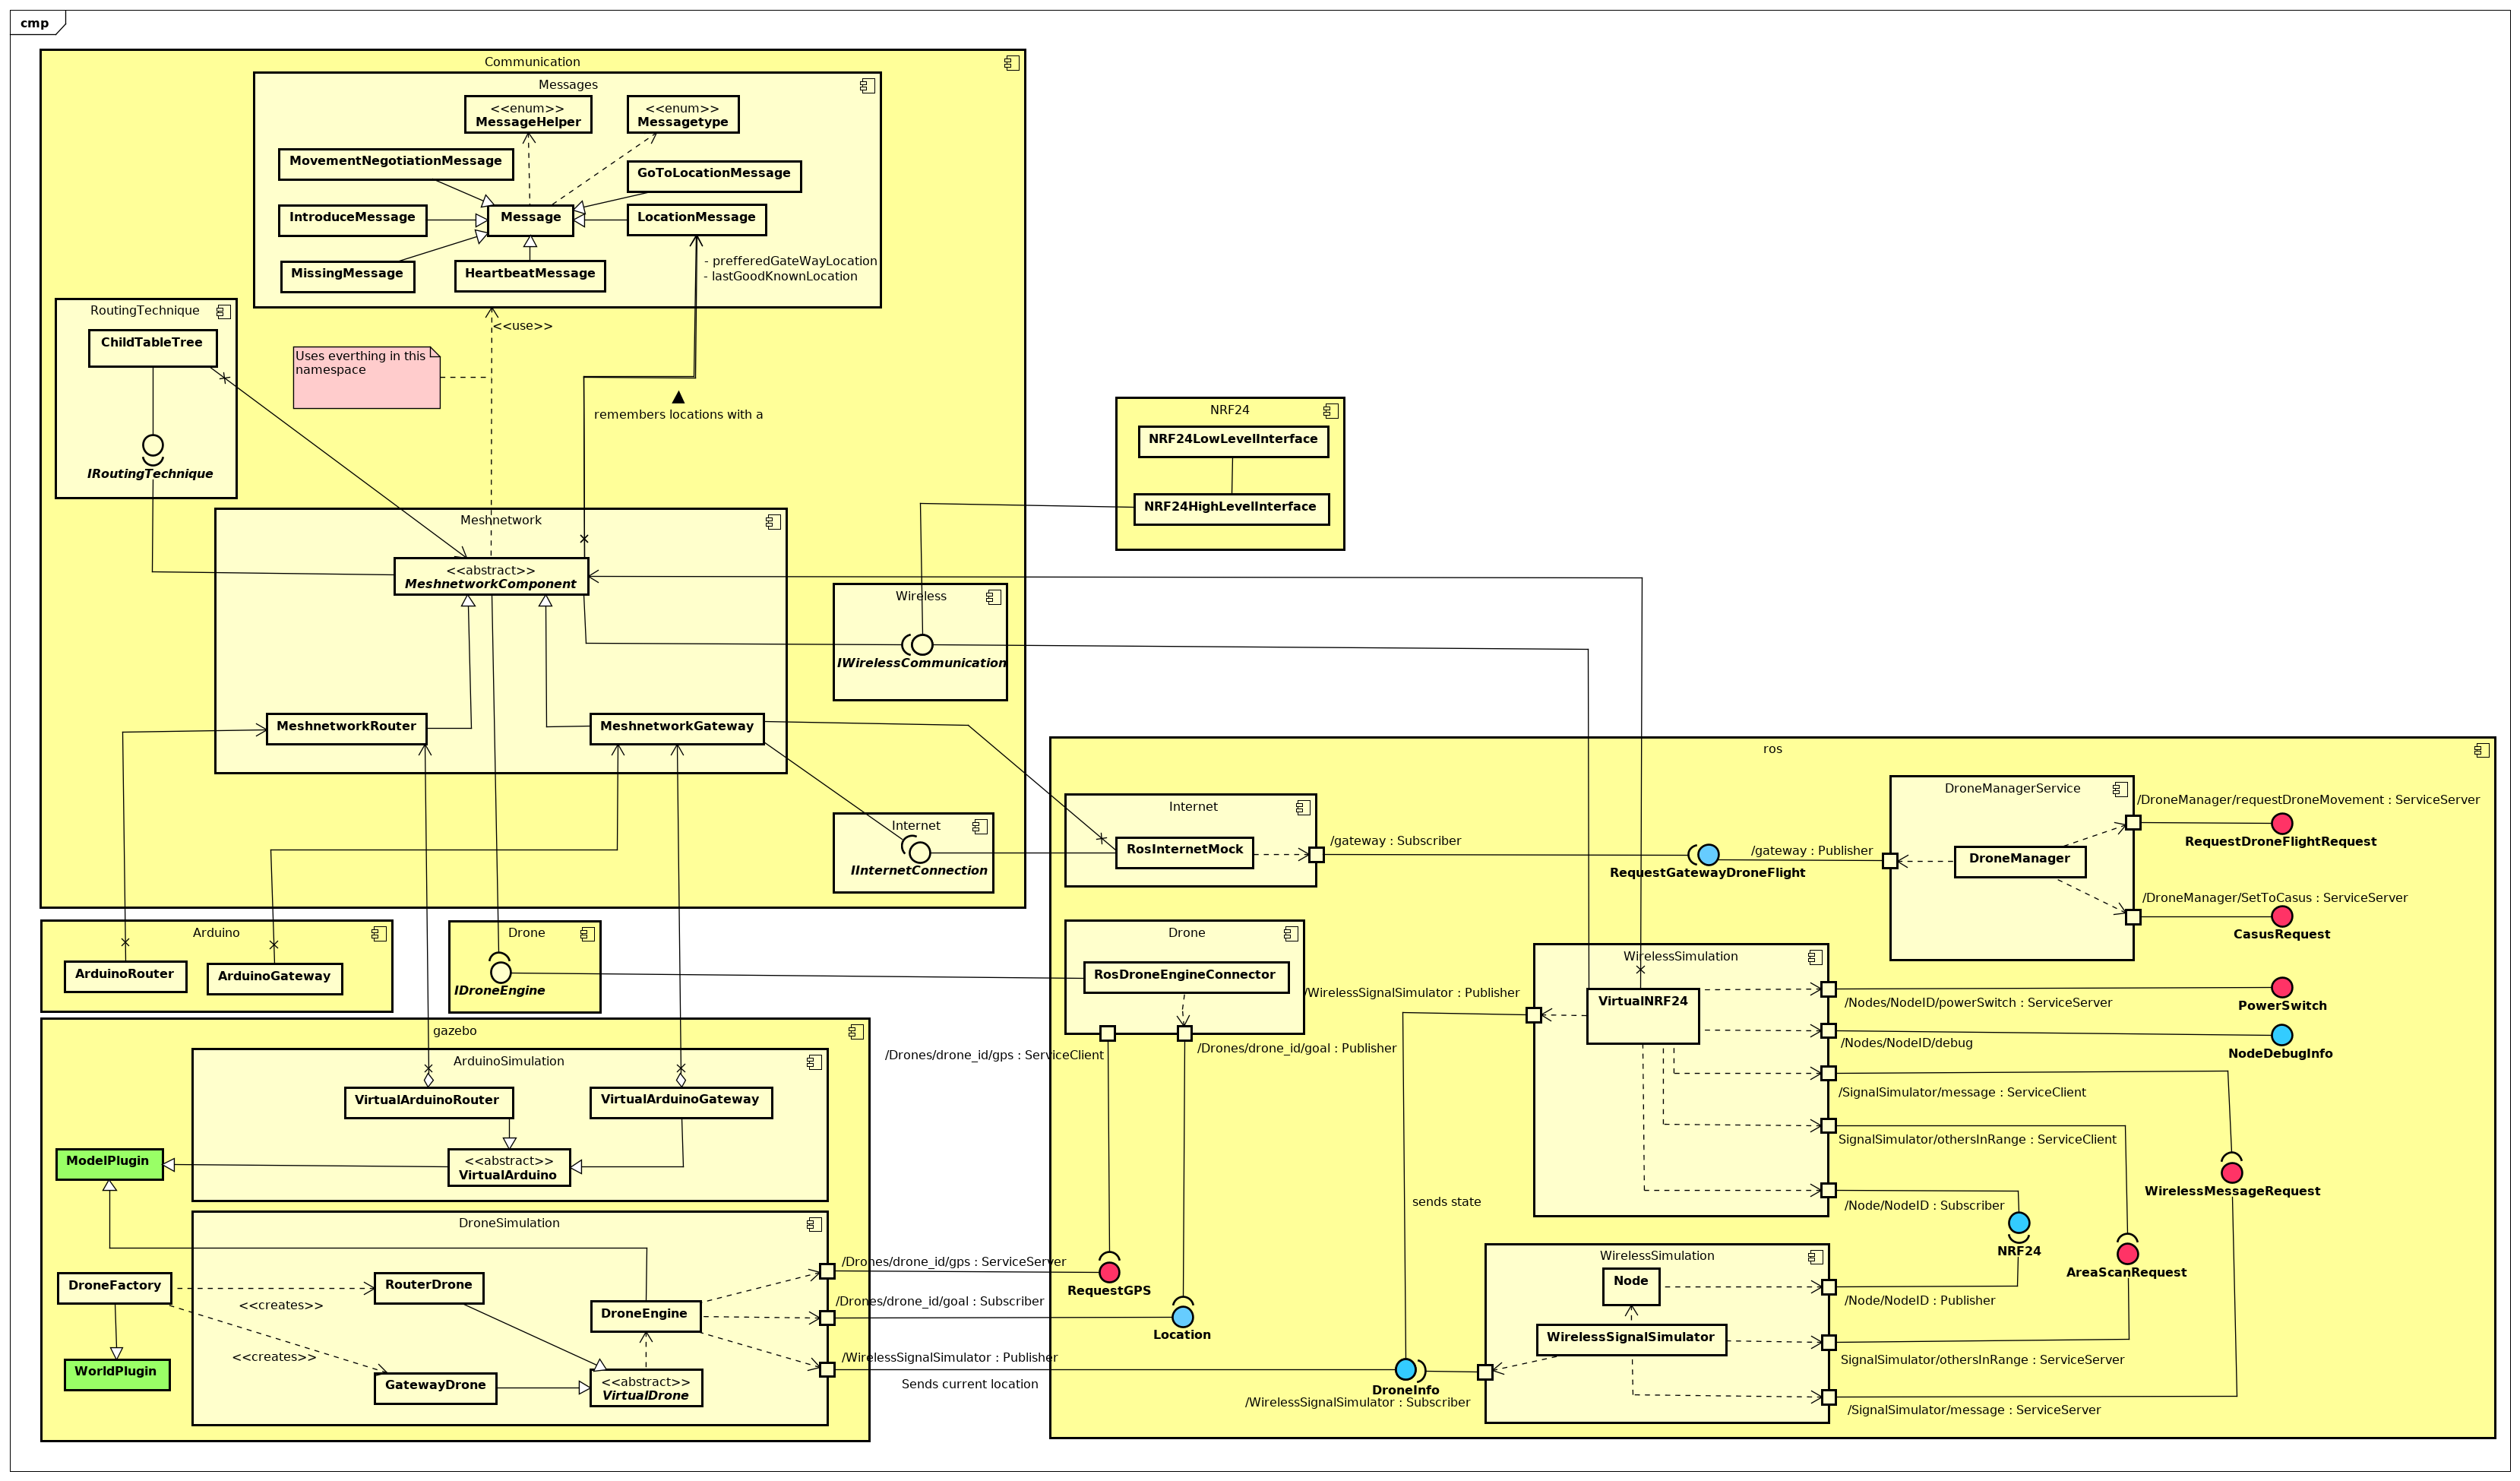
\includegraphics[width=\linewidth]{Afbeeldingen/ComponentDiagram.png}%
		\caption{package diagram drone meshnetwerk}
			\label{fig:packagediagram}
	\end{figure}%
\clearpage
\end{landscape}
\clearpage



\section{Componenten}
\label{architectural:subcomponenten}

%NAMESPACE Communication
\subparagraph{Internet}
\label{architectural:subcomponenten:Internet}
Dit component bevat alleen een high level interface om verbinding te maken en te verbreken met het internet
\subparagraph{Meshnetwork}
\label{architectural:subcomponenten:Meshnetwork}
Dit component bevat de basis componenten voor het opbouwen van een meshnetwerk.
\subparagraph{MeshnetworkComponent}
\label{architectural:subcomponenten:MeshnetworkComponent}
Een MeshnetworkComponent is de basis van elk component in het mesh netwerk.
Het vereist routeringstechniek via de \nameref{architectural:interfaces:IRoutingTechnique}, een aansluiting naar een drone via \nameref{architectural:interfaces:IDroneEngine} en een vorm van draadloze communicatie via \nameref{architectural:interfaces:IWirelessCommunication}.  Hij maakt gebruikt van het component \nameref{architectural:subcomponenten:Messages} om te communiceren met andere MeshnetworkComponenten. 
\subparagraph{MeshnetworkRouter}
\label{architectural:subcomponenten:MeshnetworkRouter}
Een meshnetwork router is een \nameref{architectural:subcomponenten:MeshnetworkComponent} die in staat is verbinding met andere nodes op te bouwen. Zijn doel is om altijd verbinding te hebben met een \nameref{architectural:subcomponenten:MeshnetworkGateway}. Als hij dit te lang niet heeft kan hij zich verplaatsen door aanspraak te maken op de DroneEngine. Wanneer hij zich in een groep van andere Routers bevind zal hij eerst onderling onderhandelen wie er zich moet verplaatsen.
\subparagraph{MeshnetworkGateway}
\label{architectural:subcomponenten:MeshnetworkGateway}
De gateway is een \nameref{architectural:subcomponenten:MeshnetworkComponent} die in staat is een verbinding op te bouwen naar een punt buiten het meshnetwerk. In de huidige situatie kan dit via een internetverbinding die loopt via de interface \nameref{architectural:interfaces:IInternetConnection}. 
\subparagraph{Messages}
\label{architectural:subcomponenten:Messages}
Dit component betreft een verzameling van bericht samenstellingen die gebruikt worden voor de communicatie van het meshnetwerk.
\subparagraph{Message}
\label{architectural:subcomponenten:Message}
Een Message is de basis van elke bericht en bevat tenminste de volgende informatie:  Maker, zender, berichttype, ontvanger, geadresseerde. 
\subparagraph{GoToLocationMessage}
\label{architectural:subcomponenten:GoToLocationMessage}
Dit bericht bevat een locatie waar een drone zich naartoe moet verplaatsen
\subparagraph{HeartbeatMessage}
\label{architectural:subcomponenten:HeartbeatMessage}
Dit bericht wordt gebruikt om de verbinding met anderen te onderhouden. Dit bericht maakt een hop per keer dat deze doorgestuurd wordt
\subparagraph{IntroduceMessage}
\label{architectural:subcomponenten:IntroduceMessage}
Een introductie bericht wordt gebruikt door een node om schik voor te stellen aan alle andere nodes die dichtbij zijn. 
\subparagraph{LocationMessage}
\label{architectural:subcomponenten:LocationMessage}
Dit bericht wordt gebruikt om de huidige locatie van een node door te sturen naar een ander.
\subparagraph{MissingMessage}
\label{architectural:subcomponenten:MissingMessage}
Zodra een \nameref{architectural:subcomponenten:MeshnetworkComponent} de verbinding verliest met een ander gebruikt hij dit bericht om andere daarover te informeren
\subparagraph{MovementNegotiationMessage}	
\label{architectural:subcomponenten:MovementNegotiationMessage}
Om onderling te onderhandelen tussen de nodes wie er actie moet ondernemen wordt dit bericht gebruikt.
\subparagraph{RoutingTechnique}
\label{architectural:subcomponenten:RoutingTechnique}
Dit component voorziet het meshnetwerk van een routing techniek wat dus inhoudt dat dit het component is die de communicatieroutes opbouwt naar andere punten in het netwerk.
  
\subparagraph{ChildTableTree}
\label{architectural:subcomponenten:ChildTableTree}
Deze techniek is een hybride meshnetwerk routing techniek waarbij een node de buren die deze heeft ziet als een kind.
Als een node een nieuw kind heeft vertelt hij dit aan zijn buren.
Omdat een node door zijn buren ook gezien wordt als kind registreren deze zijn nieuwe kind dus als kleinkind.
Hierdoor hoeft een node alleen maar te zoeken aan wie welk kind hij een bericht hoeft door te geven. 
De complexiteit van de routingtechniek neemt per stap in het netwerk af bij nodes met meerdere kinderen.
Als een drone zich verplaatst heeft wist deze het de opgebouwde geheugen van kinderen en kleinkinderen. 

\subparagraph{Wireless}
\label{architectural:subcomponenten:Wireless}
Dit component voorziet een \nameref{architectural:subcomponenten:MeshnetworkComponent} van een high level interface voor draadloze communicatie.
Als er een draadloos component wordt aangesloten moet deze hierop aangesloten worden. 

%NAMESPACE Drone
\subparagraph{Drone}
\label{architectural:subcomponenten:Drone}
Dit component representeert een drone. Omdat er op dit moment geen fysieke drone aanwezig is bezit deze component alleen een high level interface.
Deze interface is geschikt voor het ophalen van de huidige locatie en het ontvangen van een doellocatie

%NAMESPACE Arduino
\subparagraph{ArduinoRouter}
\label{architectural:subcomponenten:ArduinoRouter}
Dit component is een Arduino die voorzien is van een sketch om zich te gedragen als een router in het meshnetwerk
\subparagraph{ArduinoGateway}
\label{architectural:subcomponenten:ArduinoGateway}
Dit component is een Arduino die voorzien is van een sketch om zich te gedragen als een gateway in het meshnetwerk

%NAMESPACE GAZEBO
\subparagraph{ArduinoSimulation}
\label{architectural:subcomponenten:ArduinoSimulation}
In de dit component wordt een arduino gesimuleerd, deze simulatie is puur functioneel en betreft alleen een gelijk gedrag met betrekking tot de Arduino sketch. 
Het heeft geen effect op de clock snelheid deze is gelijk aan de computer waarop de software draait. 

\subparagraph{VirtualArduino}
\label{architectural:subcomponenten:VirtualArduino}
Dit abstracte component verplicht elke virtuele Arduino tot het aanmaken van een setup en loop functie zoals dit ook is in Arduino sketches.
Omdat deze Arduino altijd wordt toegevoegd aan een ander model erft dit component over van modelplugin.    
 
\subparagraph{VirtualArduinoRouter}
\label{architectural:subcomponenten:VirtualArduinoRouter}
Deze \nameref{architectural:subcomponenten:VirtualArduino} is voorzien van een sketch die de arduino zich laat gedragen als in router in het meshnetwerk. Dit component representeert het component \nameref{architectural:subcomponenten:ArduinoRouter} in gazebo.

\subparagraph{VirtualArduinoGateway}
\label{architectural:subcomponenten:VirtualArduinoGateway}
Deze \nameref{architectural:subcomponenten:VirtualArduino} is voorzien van een sketch die de arduino zich laat gedragen als in gateway in het meshnetwerk. Dit component representeert het component \nameref{architectural:subcomponenten:ArduinoGateway} in gazebo.


\subparagraph{DroneSimulation}
\label{architectural:subcomponenten:DroneSimulation}
Dit component is verantwoordelijk voor het simuleren van drones. 

\subparagraph{DroneEngine}
\label{architectural:subcomponenten:DroneEngine}
Elke \nameref{architectural:subcomponenten:VirtualDrone} is voorzien deze drone engine. 
Dit component maakt het mogelijk voor een drone om zich in een rechte lijn door lucht zich te verplaatsen waarbij het opstijgen en de landing verticaal wordt uitgevoerd.
Daarnaast biedt dit component via een rosservice het deel van de interface \nameref{architectural:interfaces:IDroneEngine} aan om de huidige locatie op te vragen.
Via een rostopic kan er een doel gestuurd gestuurd worden om het andere deel van de net genoemde interface te voorzien.
Tenslotte stuurt dit component bij elke verplaatsing de huidige locatie door naar de \nameref{architectural:subcomponenten:WirelessSignalSimulator}. 

\subparagraph{VirtualDrone}
\label{architectural:subcomponenten:VirtualDrone}
Een virtuele drone is een abstract component die alle variabelen bevat die nodig zijn om een drone in de wereld te injecteren. Deze variabelen betreffen een drone id, locatie en verwijzing naar de gazebo wereld. 

\subparagraph{GatewayDrone}
\label{architectural:subcomponenten:GatewayDrone}
Deze drone is een \nameref{architectural:subcomponenten:VirtualDrone} die in de sdf omschrijving wordt voorzien van een \nameref{architectural:subcomponenten:VirtualArduinoGateway} plugin. 
\subparagraph{RouterDrone}
\label{architectural:subcomponenten:RouterDrone}
Deze drone is een \nameref{architectural:subcomponenten:VirtualDrone} die in de sdf omschrijving wordt voorzien van een \nameref{architectural:subcomponenten:VirtualArduinoRouter} plugin. 

\subparagraph{DroneFactory}
\label{architectural:subcomponenten:DroneFactory}
Dit component is verantwoordelijk voor het produceren van drones. Het is een WorldPlugin die aan de hand van meegegeven parameters gateway en router drones aanmaakt.  

%NAMESPACE Ros
\subparagraph{RosDroneEngineConnector}
\label{architectural:subcomponenten:RosDroneEngineConnector}
Dit component is een adapter tussen de \nameref{architectural:subcomponenten:DroneEngine} en de interface \nameref{architectural:interfaces:IDroneEngine}. Die het mogelijk maakt om ros te gebruiken om aanspraak te maken op de virtuele drone.

\subparagraph{DroneManagerService}
\label{architectural:subcomponenten:DroneManagerService}
Dit component is de toegangspoort voor de ontwikkelaar tot de \nameref{architectural:subcomponenten:MeshnetworkGateway}.
Op dit moment is het component alleen geschikt om verplaatsingverzoeken te versturen via de gateway naar de Drones.
Hiervoor biedt het twee interfaces in de vorm van rosservices aan waarbij er een voor locaties is en de ander voor casussen. 

\subparagraph{DroneManager}
\label{architectural:subcomponenten:DroneManager}
Dit subcomponent realiseert de rosservices en publiceert verplaatsingverzoeken naar de gateways.  

\subparagraph{RosInternetMock}
\label{architectural:subcomponenten:RosInternetMock}
Deze internetmock laat de \nameref{architectural:subcomponenten:DroneManager} zich voordoen als internetpunt zodat er geen daadwerkelijke TCP/IP implementatie hoeft worden gemaakt 
\subparagraph{WirelessSimulation}
\label{architectural:subcomponenten:WirelessSimulation}
Het WirelessSimulation component is verantwoordelijk voor het simuleren van de NRF24 en het draadloze signaal hiervan. 
\subparagraph{WirelessSignalSimulator}
\label{architectural:subcomponenten:WirelessSignalSimulator}
Deze simulator bepaald of twee nodes met elkaar mogen communiceren. Het doet dit op basis van informatie die het continue ontvangt via het drone informatie topic. 
\subparagraph{Node}
\label{architectural:subcomponenten:Node}
Dit component wordt alleen gebruikt door de \nameref{architectural:subcomponenten:WirelessSignalSimulator} om te registreren welke Nodes bestaan, waar ze zijn en naar welk topic ze luisteren.
\subparagraph{VirtualNRF24}
\label{architectural:subcomponenten:VirtualNRF24}
Dit component is de virtuele versie van de NRF24, het is in staat om payloads te verwerken van 32 byte.
Deze kan de NRF24 naar een direct adres versturen of zenden naar alle NRF24 nodes binnen bereik.

\section{Interfaces}
\label{architectural:interfaces}
\subparagraph{IInternetConnection}
\label{architectural:interfaces:IInternetConnection}
Deze high level interface wordt gebruikt voor het leggen van een verbinding naar een extern punt buiten het netwerk. Omdat de gateway zich alleen hoeft te verbinden met een punt bestaat deze interface alleen uit een connect() en een disconnect().
\subparagraph{IWirelessCommunication}
\label{architectural:interfaces:IWirelessCommunication}
In deze interface wordt de functionaliteit gesteld waar een draadloos communicatiemiddel aan moet voldoen. Het bevat functies om een antenne te starten en te stoppen. Het versturen van een bericht naar een specifiek punt of het zenden naar elke punt in de buurt. Er is een functie aanwezig om wanneer mogelijk debugging te gebruiken. Tenslotte moet een aansluitend component met deze interface moeten kunnen teruggeven of deze aan of uit staat.

\subparagraph{NRF24HighLevelInterface}
\label{architectural:interfaces:NRF24HighLevelInterface}

Deze high level interface is de aangeboden interface van de NRF24 en voldoet aan de interface \nameref{architectural:interfaces:IWirelessCommunication}. Het praat direct met de driver van de NRF24.  

\subparagraph{NRF24LowLevelInterface}
\label{architectural:interfaces:NRF24LowLevelInterface}
Deze low level interface is de driver van de NRF24


\subparagraph{IDroneEngine}
\label{architectural:interfaces:IDroneEngine}
Een drone engine interface representeert de aansluiting met een drone.
Hierin moet het mogelijk zijn om een doel coördinaat te sturen naar de drone om zich naartoe te verplaatsen. 
Daarnaast moet het mogelijk zijn voor een drone om de huidige positie terug te geven.
\subparagraph{IRoutingTechnique}
\label{architectural:interfaces:IRoutingTechnique}
Deze interface bevat functies voor het uitvoeren van een routeringstechniek.
Het heeft functies voor het starten en onderhouden van het netwerk.
Daarnaast zijn er functies hoe gereageerd moet worden op het vinden en verliezen van andere netwerkpunten.
Er zijn functies aanwezig om een adres op te halen waar naartoe gezonden moet worden om een punt te bereiken.
Ook kan er opgehaald worden welke punten zijn aangesloten, hoeveel punten dit zijn en hoeveel directe aansluitingen er zijn.
Tenslotte is er functie aanwezig die aangeroepen wordt zodra een drone zich verplaatst zodat hier adequaat op gereageerd kan worden.

\section{Ros topics en services}
\label{architectural:ros_service_topic}
Zoals al eerder benoemd wordt er gebruik gemaakt van de transportlaag van ROS. Dit wordt gedaan in de vorm van Ros topics en services. Hieronder worden de messages en services kort toegelicht.

\subparagraph{RequestGatewayDroneFlight}
\label{architectural:ros:RequestGatewayDroneFlight}

\subparagraph{CasusRequest}
\label{architectural:ros_service:CasusRequest}

\subparagraph{PowerSwitch}
\label{architectural:ros_service:PowerSwitch}

\subparagraph{WirelessMessageRequest}
\label{architectural:ros_service:WirelessMessageRequest}

\subparagraph{AreaScanRequest}
\label{architectural:ros_service:AreaScanRequest}

\subparagraph{RequestGPS}
\label{architectural:ros_service:RequestGPS}

\chapter{Detailed Design Description}
\label{DetailedDesign}
\section{Deployment Diagram}
\label{DetailedDesign:deployment}
De volgende paragraaf behandeld het deployment diagram 



\subsection{Design Decisions related to deployment}
\label{DetailedDesign:deployment:decisisions}
\section{Design Sub-Systeem Drone Simulatie}
\label{DetailedDesign:DroneSimumlatie}
\subsection{Design Class Diagram}
\label{DetailedDesign:DroneSimumlatie:class}
\begin{figure}[H]
	\begin{center}\includegraphics[width=\linewidth]{UML/out/DroneSimulation/class/DroneSimClass/DroneSimClass.png}\end{center}
	\caption{class diagram Drone Simulatie}
	\label{fig:class:dronesimulatie}
\end{figure}
\subsection{Sequence Diagrams}
\label{DetailedDesign:DroneSimumlatie:sequence}
\subsection{Activity and State Diagrams}
\label{DetailedDesign:DroneSimumlatie:Activity}
\subsection{Design decisions made for the sub-system}

\section{Design Sub-Systeem Meshnetwerk}
\label{DetailedDesign:MeshNetwerk}
\subsection{Design Class Diagram}
\label{DetailedDesign:MeshNetwerk:class}
\label{DetailedDesign:DroneSimumlatie:class}
%\begin{figure}[H]
%	\begin{center}\includegraphics[width=\linewidth]{UML/out/MeshNetwork/class/DroneSimClass/DroneSimClass.png}\end{center}
%	\caption{class diagram Drone Simulatie}
%	\label{fig:class:dronesimulatie}
%\end{figure}
\subsection{Sequence Diagrams}
\label{DetailedDesign:MeshNetwerk:sequence}
\subsection{Activity and State Diagrams}
\label{DetailedDesign:MeshNetwerk:activity}
\subsection{Design decisions made for the sub-system}
\label{DetailedDesign:MeshNetwerk:decisions}

\section{Design Sub-System Wireless Simulatie}
\label{DetailedDesign:WirelessSimulatie}
\subsection{Design Class Diagram}
\label{DetailedDesign:WirelessSimulatie:class}
\subsection{Sequence Diagrams}
\label{DetailedDesign:WirelessSimulatie:sequence}
\subsection{Activity and State Diagrams}
\label{DetailedDesign:WirelessSimulatie:activity}
\subsection{Design decisions made for the sub-system}
\label{DetailedDesign:WirelessSimulatie:decisions}


\bibliographystyle{apacite}
\bibliography{bilbliography.bib}

\clearpage
\appendix
\chapter{Appendix 1}
\label{app:iteratieplan}





\end{document}